%% LyX 2.1.3 created this file.  For more info, see http://www.lyx.org/.
%% Do not edit unless you really know what you are doing.
\documentclass[english]{article}
\usepackage[T1]{fontenc}
\usepackage[latin9]{inputenc}
\usepackage{array}
\usepackage{amsmath}
\usepackage{cancel}
\usepackage{graphicx}

\makeatletter

%%%%%%%%%%%%%%%%%%%%%%%%%%%%%% LyX specific LaTeX commands.
%% Because html converters don't know tabularnewline
\providecommand{\tabularnewline}{\\}

\makeatother

\usepackage{babel}
\begin{document}

\title{Hall Effect}


\author{Atul Singh Arora}


\date{March 2015}

\maketitle

\section{Theory}

Assuming the Drude model, it can be shown that (see for example Ashcroft
and Mermin) the equation of motion per electron becomes 
\[
\frac{dp}{dt}=-\frac{p}{\tau}+f
\]
where $f$ is the force, and $\tau$ is s.t. probability of collision
of an electron in time $dt$ is $dt/\tau$. Let us now consider the
situation depicted by the following diagram {[}taken from Ashcroft
and Mermin{]}. It seems reasonable to imagine that for a fixed value
of $E_{x}$, $j_{x}$ will depend on $H$ by adding to the resistance
in some way. We therefore define a quantity\footnote{Recall: In general, we define $\rho$ as $\mathbf{E}=\rho\mathbf{j}$.
If we consider a typical case (straight wire), we get $j=I/A$, $V=EL$
and get $V=I\rho L/A$ which using ohms definition, we get the familiar
$R=\rho L/A$}, Magneto-resistance as 
\[
\rho(H)=\frac{E_{x}}{j_{x}}
\]
which was experimentally found by Hall to indeed by field dependent.
Next since by inspection we already know that in steady state, $E_{y}$
must balance the lorentz force, which is proportional to both $H$
and to $j_{x}$, we define a quanitity known as the Hall coeffecient
\[
R_{H}=\frac{E_{y}}{j_{x}H}
\]
At this very step, one can make a rather important point. The direction
of $E_{y}$ depends on whether the charge of the current mediator
is positive or negative. If the charge is negative, as shown below,
$E_{y}$ will be negative, and therefore so will $R_{H}$. If the
charge were positive, $R_{H}$ will be positive.

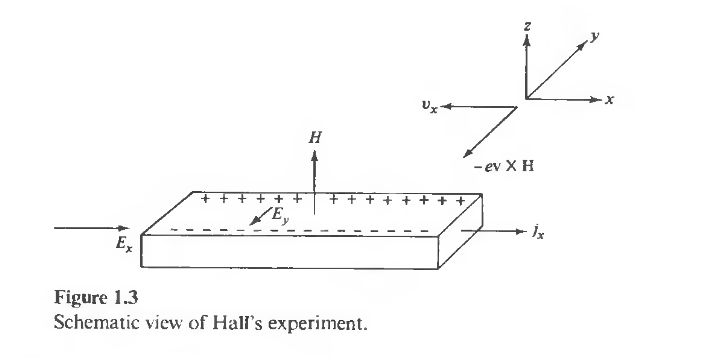
\includegraphics[bb=0bp 60bp 703bp 357bp,clip,width=16cm]{diagram}

We now derive these quantities under the Drude model. Let's start
with using the equation of motion per electron for an arbitrary $E$
and $B$ field as 
\[
\frac{d\mathbf{p}}{dt}=-e\left(\mathbf{E}+\frac{\mathbf{p}}{mc}\times\mathbf{H}\right)-\frac{\mathbf{p}}{\tau}
\]
In the steady state then, for the given set of fields, we'll have
\[
\begin{aligned}0= & -eE_{x}+\cancelto{-\omega_{c}p_{y}}{\left(-\frac{eH}{mc}p_{y}\right)}-\frac{p_{x}}{\tau}\\
0= & -eE_{y}-\cancelto{-\omega_{c}p_{x}}{\left(-\frac{eH}{mc}p_{y}\right)}-\frac{p_{y}}{\tau}
\end{aligned}
\]
Recall case: Only $\mathbf{E}$ fields: 
\begin{itemize}
\item $\rho$ is defined as$\mathbf{E}\equiv\rho\mathbf{j}$, and $\sigma\equiv1/\rho$
\item $\mathbf{j}=-ne\mathbf{v}$ (where $n$ is the number of electrons
per unit volume)
\item In the presence of only a constant $\mathbf{E}$ field, we have 
\[
\mathbf{v}=-\frac{ne\mathbf{E}\tau}{m}
\]
which entails 
\[
\mathbf{j}=\frac{-ne^{2}\tau}{m}\mathbf{E}=\sigma\mathbf{E}
\]
thus 
\[
\sigma=\frac{ne^{2}\tau}{m}
\]

\end{itemize}
Getting back to the equations, we multiply by 
\[
-\frac{ne\tau}{m}
\]
 to get
\[
\begin{aligned}\sigma_{0}E_{x}= & \omega_{c}\tau j_{y}+j_{x}\\
\sigma_{0}E_{y}= & -\omega_{c}\tau j_{x}+j_{y}
\end{aligned}
\]
where $\mathbf{j}=-ne\mathbf{p}/m$. Next we assume that in steady
state, $j_{y}$ is zero. Plugging this in the previous equations we
get
\[
\begin{aligned}\sigma_{0}E_{x}= & j_{x} & \implies E_{x}= & j_{x}\left(\frac{m}{ne^{2}\tau}\right)=j_{x}\rho & \implies & \rho(H)=\frac{m}{ne^{2}\tau}\\
\sigma_{0}E_{y}= & -\omega_{c}\tau j_{x} & \implies E_{y}= & -j_{x}\frac{\cancel{e}H}{\cancel{m}c}\cancel{\tau}\frac{\cancel{m}}{ne^{\cancel{2}}\cancel{\tau}}=j_{x}\left(-\frac{1}{nec}\right)H=j_{x}R_{H}H & \implies & R_{H}=-\frac{1}{nec}
\end{aligned}
\]
So in accordance with our theory, $\rho(H)$ doesn't dependent on
$H$, the field. This can be verified experimentally. Further, it
depends on $\tau$ which can depend on various parameters, including
temperature. 

However, $R_{H}$ according to the theory is rather boldly predicted
to be independent of all parameters of the metal, except the electron
density. This density can be calculated assuming that only the valence
electrons of the metal participate in the process of metallic conduction.
However, experimentally it is known that $R_{H}$ does depend on the
field strength $H$.


\section{Experimental Setup}

The 

FAQ: 

1. Write about how you would fix the issue: magnetic field in the
centre is non zero

2. Even at zero magnetic field, the multimeter reads non-zero current
(this is ``hall current'')


\subsection{Observations}


\subsubsection{Time-line}

\begin{tabular}{llp{9cm}}
\hline 
March 20 & Friday & Started and almost finished performing the experiment\tabularnewline
March 23 & Monday & Understood whether or not repeating is required (longitudenal voltage)
| started writing the record\tabularnewline
March 24 & Tuesday & Completed the record and analyzed the data and worked on writing the
record\tabularnewline
\hline 
\end{tabular}
\end{document}
